\section{Theorie}
\label{sec:Theorie}


\subsection{Aufbau eines Koaxialkabels}
Das Koaxialkabel ist eine Datenübertragungsleitung, die aus mehreren Schichten aufgebaut ist. 
\autoref{fig:koax} zeigt diesen Aufbau anhand eines geöffneten Kabels.
\begin{figure}
    \centering
    
\includegraphics[width=\textwidth]{koax.png}
    \caption{Querschnitt eines Koaxialkabels~\cite[S]{quelle}}
    \label{fig:koax}
\end{figure}
\FloatBarrier\noindent
Den Kern eines Koaxialkabels bildet der Innenleiter, über den das Signal gesendet wird. 
Es folgt ein Dielektrikum zur Isolierung des Innenleiters gegen die anderen Komponenten.
Die nächste Schicht ist die Abschirmung, die verschiedene Gestalt haben kann und ebenfalls elektrisch leitend ist.
Durch die Abschirmung wird das gespiegelte Signal gesendet.
Die durch den Stromfluss entstehenden Magnetfelder heben sich daher auf, was das Kabel sehr rauscharm macht.
Die äußerste Schicht bildet der Kabelmantel, der das Kabel gegen mechanische Einwirkung und Kurzschlüsse schützt.
\subsection{Signalübertragung auf verlustbehafteten Leitungen}
Reale Leitungen sind verlustbehaftet und können mithilfe eines Ersatzschaltbilds modelliert werden, was \autoref{fig:schaltung} zeigt.
\begin{figure}
    \centering
    
\includegraphics[width=\textwidth]{ersatzschaltbild.png}
    \caption{Ersatzschaltbild einer verlustbehafteten Leitung~\cite[1]{v52}.}
    \label{fig:schaltung}
\end{figure}
\FloatBarrier\noindent
Die Verluste werden beschrieben durch eine Kapazität $C$ zwischen Innen- und Aussenleiter, der Induktivität $L$, den Widerstandsbelag $R$, und den Querleitbelag $G$.
Letzterer gibt an, wie groß die Verluste durch Stromfluss durch das Diekeltrikum sind.
Für die gute Funktion von Koaxialkabeln ist es wichtig, dass kein Strom im Dielektrikum fließt.
Daher ist bei diesen Leitungen $G\approx 0$ und die Ohm'schen Verluste überwiegen.\\
Das Verhalten bei Anlegen einer Signalspannung liefert die Telegrafengleichung
\begin{equation*}
    \frac{\partial^2U}{\partial t^2} = LC\frac{\partial^2U}{\partial t^2} + \left(LG + RC\right)\frac{\partial U}{\partial t} + RGU.
\end{equation*}
Die Lösungen sind gedämpfte harmonische Schwingungen der Form
\begin{equation*}
    U(z,t)= U\symup{e}^{-\gamma z}\symup{e}^{i\omega t}
\end{equation*}
mit der Ausbreitungskonstante
\begin{equation*}
    \gamma = \sqrt{\left(R+i\omega L\right)\left(G+i\omega C\right)} = \alpha + i\beta.
\end{equation*}
Die 
%
%
%
\subsection{Leitungsverluste durch den Skin-Effekt}
Der Skin-Effekt beschreibt die Erhöhung des Widerstandsbelags bei hohen Frequenzen ab $f=\qty{100}{\kilo\hertz}$.
Der Stromfluss im Leiter erzeugt Wirbelströme, die den Wechselstrom des Signals verdrängen und so den effektiven Wirkungsquerschnitt verringern.
Dies führt zum Anstieg des Widerstandsbelags.
Bei den Frequenzen, bei denen der Skin-Effekt relevant wird, ist die Proportionaliät ungefähr $R\propto \sqrt{\omega}$.
%
%
\begin{equation}
    \left|Z\right| = \sqrt{R^2+\omega^2 L^2}
    \label{eqn:impedanz}
\end{equation}
%
%
%
\begin{equation}
    \mathrm{tan}\left(\varphi\right) = \frac{\omega L}{R}
    \label{eqn:phase}
\end{equation}
Diese Formeln hatte sie uns gegeben, aber man findet bestimmt auch nh Quelle.
% 
%
%
%
%
\begin{equation}
    L = \frac{v_{\mathrm{Phase}} \Delta t}{2}
    \label{eqn:laenge}
\end{equation}
%
%
%
%
\begin{equation}
    v_{\mathrm{Phase}} = \frac{c_0}{\sqrt{\epsilon_r}}
    \label{eqn:phasengeschw}
\end{equation}
%
%
%
%
\begin{equation}
    \alpha = \frac{1}{2l} \mathrm{ln}\left(\frac{U_0}{U_l}\right)
    \label{eqn:daempfung}
\end{equation}
Faktor 2 wegen hin und Rückweg. Kann die Formel zur not auch in die Auswertung übernehemen. ergibt sich aus:
\begin{equation*}
    U\left(l\right) = U_0 \mathrm{exp}\left(-\alpha l\right)
\end{equation*}
%
%
%
%
\begin{equation}
    \epsilon_r = \left(\frac{c_0 \Delta t}{2 l}\right)^2
    \label{eqn:diel}
\end{equation}
%
%
%
%
\begin{figure}
        \centering
        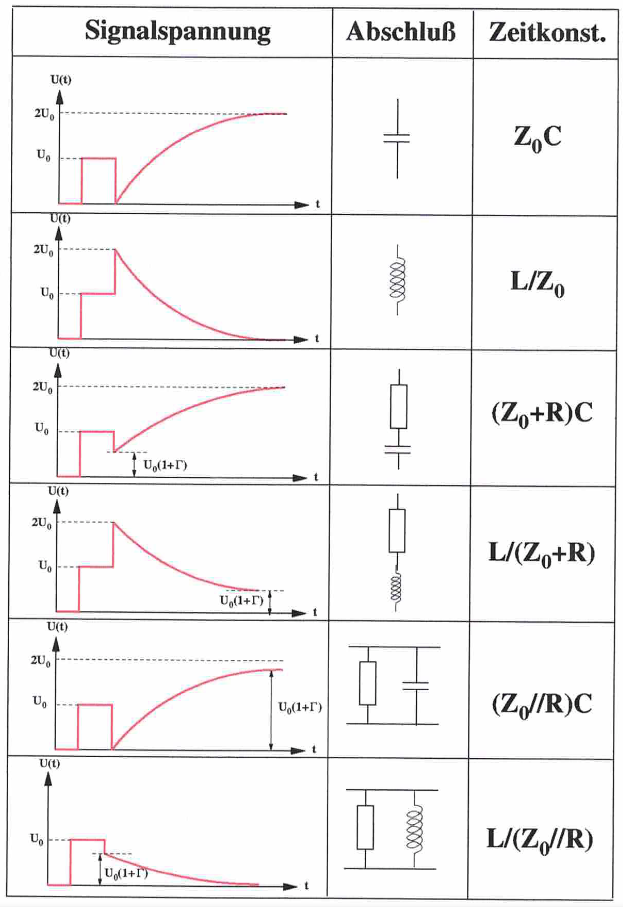
\includegraphics[width=0.5\textwidth]{content/images/signalspannungen.png}
        \caption{Erwartete Signalspannungen bei entsprechendem Abschluss sowie zugehörige Zeitkonstante \cite{V52}.}
        \label{fig:signalspannungen}
\end{figure}
%
%
%
\subsection{Relative Abweichung experimenteller Messwerte}
Zur Berechnung der relativen Abweichung von experimentell bestimmten Werten zu theoretischen Werten wird 
\begin{equation}
    \increment x_{\mathrm{rel}} = \left| \frac{x_{\mathrm{exp}}-x_{\mathrm{theo}}}{x_{\mathrm{theo}}}\right|
    \label{eqn:relabw}
\end{equation}
verwendet \cite{relabw}. 

